\documentclass{beamer}

\mode<presentation> {

% The Beamer class comes with a number of default slide themes
% which change the colors and layouts of slides. Below this is a list
% of all the themes, uncomment each in turn to see what they look like.

%\usetheme{default}
%\usetheme{AnnArbor}
%\usetheme{Antibes}
%\usetheme{Bergen}
%\usetheme{Berkeley}
%\usetheme{Berlin}
%\usetheme{Boadilla}
%\usetheme{CambridgeUS}
%\usetheme{Copenhagen}
%\usetheme{Darmstadt}
%\usetheme{Dresden}
%\usetheme{Frankfurt}
%\usetheme{Goettingen}
%\usetheme{Hannover}
%\usetheme{Ilmenau}
%\usetheme{JuanLesPins}
%\usetheme{Luebeck}
\usetheme{Madrid}
%\usetheme{Malmoe}
%\usetheme{Marburg}
%\usetheme{Montpellier}
%\usetheme{PaloAlto}
%\usetheme{Pittsburgh}
%\usetheme{Rochester}
%\usetheme{Singapore}
%\usetheme{Szeged}
%\usetheme{Warsaw}

% As well as themes, the Beamer class has a number of color themes
% for any slide theme. Uncomment each of these in turn to see how it
% changes the colors of your current slide theme.

%\usecolortheme{albatross}
%\usecolortheme{beaver}
%\usecolortheme{beetle}
%\usecolortheme{crane}
%\usecolortheme{dolphin}
%\usecolortheme{dove}
%\usecolortheme{fly}
%\usecolortheme{lily}
%\usecolortheme{orchid}
%\usecolortheme{rose}
%\usecolortheme{seagull}
%\usecolortheme{seahorse}
%\usecolortheme{whale}
%\usecolortheme{wolverine}

%\setbeamertemplate{footline} % To remove the footer line in all slides uncomment this line
%\setbeamertemplate{footline}[page number] % To replace the footer line in all slides with a simple slide count uncomment this line

%\setbeamertemplate{navigation symbols}{} % To remove the navigation symbols from the bottom of all slides uncomment this line
}

\usepackage{graphicx, graphics}
\usepackage{booktabs}
\usepackage{ulem, cancel}
\usepackage{multicol}
\setlength{\columnseprule}{0.4pt}
\usepackage{tcolorbox}
\DeclareGraphicsExtensions{.pdf,.png,.jpg,.gif}

\title[UNIST \LaTeX]{\LaTeX\ Lecture for UNIST}

\author{Jaewoong Lee}
\institute[UNIST]
{
Ulsan National Institute of Science and Technology
\medskip
\newline
\textit{jwlee230@unist.ac.kr}
}
\date{\today} % Date, can be changed to a custom date

\begin{document}

\begin{frame}
\titlepage
\end{frame}

\begin{frame}
\frametitle{Overview}
\tableofcontents
\end{frame}

\section{Introduction myself}

\begin{frame}
    \frametitle{I am...}
    \begin{itemize}
        \item Jaewoong Lee
        \item Senior at UNIST
        \item \LaTeX\ user since 2014
        \item Graduated Gyeonggi Science High School for the Gifted in 2016
        \item Full Member of GSHS TeX User Association
    \end{itemize}
    \begin{figure}[h!]
        \centering
        
\includegraphics[width=0.7 \textwidth]{figures/gshs-tex.png}
        \caption{GSHS TeX User Association}
    \end{figure}
\end{frame}

\begin{frame}
    \frametitle{What you could with \LaTeX?}
    From a simple report to a presentation. \\
    This presentation file is also made by \LaTeX. \\
    You can do almost everything in written form.
\end{frame}

\begin{frame}
    \frametitle{Refer this page}
    {\LARGE \url{https://fumire.moe/Lecture/latex/} \\}
    You can easily get TeX code in this lecture from here!
\end{frame}

\section{What is \LaTeX?}

\begin{frame}
    \frametitle{\LaTeX?}
    \begin{itemize}
        \item LAH-tekh or LAY-tekh
        \item TeX-like editing tool
        \item In simple, that which is making a paper.
        \item Donald Knuth made TeX $\Rrightarrow$ \LaTeX: a macro for TeX
        \item WYSIWYM
    \end{itemize}
\end{frame}

\begin{frame}
    \frametitle{WYSIWYG vs. WYSIWYM}
    \begin{columns}[c]
        \column{.45 \textwidth}
        \textbf{WYSIWYG}
        \begin{itemize}
            \item What you see is what you get
            \item MS Word or HWP
        \end{itemize}
        
        \column{.5 \textwidth}
        \textbf{WYSIWYM}
        \begin{itemize}
            \item What you see is what you mean
            \item HTML, \LaTeX
        \end{itemize}
    \end{columns}
\end{frame}

\begin{frame}
    \frametitle{\LaTeX\ \textit{(cont.)}}
    \begin{itemize}
        \item You write the contents, then \LaTeX makes it!\
        \item Useful to write an equation
        \item As an equation editor, \LaTeX\ is a \textit{de facto} standard
        \item Convenient labeling \& referencing
        \item After initial setting, you only think about contents; not design
        \item Table of contents, List of figures? $\Rrightarrow$ Only one line command!
        \item Cross-referencing: 'As figure 8a' $\Rrightarrow$ You can see 'Big Picture'
        \item Easily attach vector image like SVG \& PDF
    \end{itemize}
\end{frame}

\begin{frame}
    \frametitle{\LaTeX\ vs. MS word}
    \begin{figure}[h!]
        \centering
        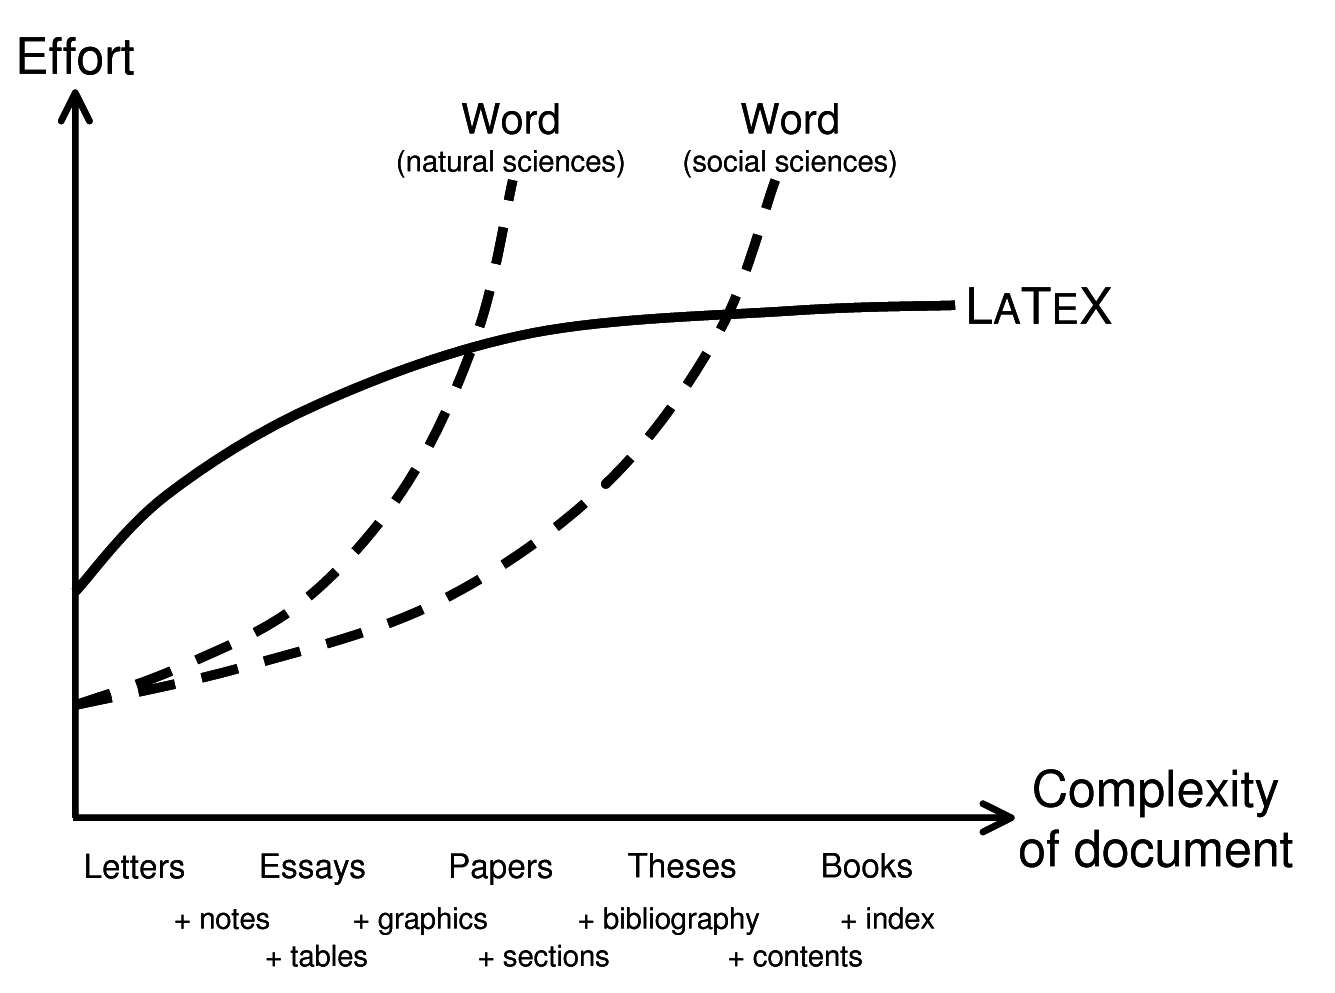
\includegraphics[width=.5 \linewidth]{figures/texvsword.jpg}
        \caption{\LaTeX\ vs. MS word}
    \end{figure}
\end{frame}

\begin{frame}
    \frametitle{\LaTeX\ vs. MS word \textit{(cont.)}}
    \begin{itemize}
        \item \LaTeX\ users were slower than Word users.
        \item \LaTeX\ users wrote less text in the same amount of time.
        \item \LaTeX\ users produced more typesetting, orthographical, grammatical, and formatting errors. 
        \item \LaTeX\ users more often report enjoying using their respective software.
    \end{itemize}
    According to Knauff, M., \& Nejasmic, J. (2014). An efficiency comparison of document preparation systems used in academic research and development. PloS one, 9(12), e115069.
\end{frame}

\section{Hello World Example}

\begin{frame}[fragile]
    \frametitle{Hello World for \LaTeX}
    \begin{columns}[c]
        \column{.45 \textwidth}
        \begin{example}[Hello World]
            \begin{verbatim}
\documentclass{article}
\title{Hello world}
\author{John Doe}
\date{September 2019}
\begin{document}
\maketitle
Lorem ipsum dolor sit amet.
\end{document}
            \end{verbatim}
        \end{example}
        
        \column{.5 \textwidth}
        \begin{enumerate}
            \item This is an article.
            \item The title is 'Hello world'.
            \item The author is 'John Doe'.
            \item Written in September 2019.
            \item This document contains a title and a sentence.
        \end{enumerate}
    \end{columns}
\end{frame}

\section{Introduction to \LaTeX}

\begin{frame}
    \frametitle{Structure of \LaTeX}
    Preamble
    \begin{itemize}
        \item In simple, a header of document.
        \item Declare class of document, packages, \textit{et cetera}.
        \item Make a declaration of settings, also.
    \end{itemize}
    Body
    \begin{itemize}
        \item Whole thing after \texttt{\textbackslash begin\{document\}}
        \item Similar as editing mode in Wikipedia.
    \end{itemize}
\end{frame}

\begin{frame}
    \frametitle{Hierarchy of Document}
    \begin{enumerate}
        \item \textbackslash document
        \item \textbackslash part
        \item \textbackslash chapter
        \item \textbackslash section
        \item \textbackslash subsection
        \item \textbackslash subsubsection
        \item \textbackslash paragraph
        \item \textbackslash subparagraph
    \end{enumerate}
\end{frame}

\begin{frame}[fragile]
    \frametitle{Table of Contents}
    Only one line command is required to make 'Table of Contents'.
    \begin{example}[ToC code]
        \begin{verbatim}
\documentclass{article}
\begin{document}
    \tableofcontents
    \section{one}
    \subsection{two}
\end{document}
        \end{verbatim}
    \end{example}
    As the example, just add \texttt{\textbackslash tableofcontents} command where you want.
\end{frame}

\begin{frame}[fragile]
    \frametitle{Special Characters}
    You cannot use these character directly: 
    \begin{block}{Special Characters}
        \textbackslash, \#, \$, \%, \&, \{, \}, \_
    \end{block}
    As following block, this problem has been solved by adding backslash in front of the character:
    \begin{block}{Using Special Characters}
        \textbackslash textbackslash, \textbackslash\#, \textbackslash\$, \textbackslash\%, \textbackslash\&, \textbackslash\{, \textbackslash\}, \textbackslash\_
    \end{block}
    Moreover, \% means one line comment in \LaTeX. Please refer here\footnotemark\ when you want multiple line comment.
    
    \footnotetext{http://bit.ly/2iZi3yn}
\end{frame}

\begin{frame}
    \frametitle{Spacing \& Line Break}
    Even if there are so many spaces in \LaTeX\ code, there is only one space in the result. If you want to use many spaces, use '\texttt{\textbackslash\ }' instead. \\
    In the same way, there are so many line breaks in \LaTeX\ code, there is only one line break. When you want to line breaks, use '\texttt{\textbackslash\textbackslash}' instead. \\
    Furthermore, twice of line break start new paragraph in \LaTeX.
\end{frame}

\begin{frame}[fragile]
    \frametitle{Page Break}
    Use \texttt{\textbackslash newpage} or \texttt{\textbackslash clearpage}.\\
    When make a book, use \texttt{\textbackslash cleardoublepage}.
\end{frame}

\begin{frame}[fragile]
    \frametitle{Text Aligning}
    \begin{flushleft}
        Align Text Left. Use \texttt{flushleft}.
    \end{flushleft}
    \begin{center}
        Justify Text. Use \texttt{center}.
    \end{center}
    \begin{flushright}
        Align Text Right. Use \texttt{flushright}.
    \end{flushright}

    In using \texttt{flushleft}, \texttt{center} or \texttt{flushright}, please refer following:
    \begin{block}{Text Aligning}
        \begin{verbatim}
\begin{flushright}
Right Aligned Text is here.
\end{flushright}
        \end{verbatim}
    \end{block}
\end{frame}

\begin{frame}[fragile]
    \frametitle{Text Color}
    This example shows different examples on how to user the \texttt{xcolor} package to change the color of elements in \LaTeX.
    
    \begin{columns}[c]
        \column{.45 \textwidth}
        \begin{example}[xcolor code]
            \begin{verbatim}
\documentclass{article}
\usepackage{xcolor}
\begin{document}
\textcolor{green}
    {Hello,}
\colorbox{orange}
    {world!}
\end{document}
            \end{verbatim}
        \end{example}
        
        \column{.5 \textwidth}
        \begin{example}[color showing]
            \textcolor{green}{Hello,}
            \colorbox{orange}{world!}
        \end{example}
        
    \end{columns}
    
\footnotetext{Reference: http://bit.ly/2UssO6a}
\end{frame}

\begin{frame}
    \frametitle{Font Styles}
    \begin{itemize}
        \item \textbf{Bold}: \texttt{\textbackslash textbf\{...\}}
        \item \textit{Italic}: \texttt{\textbackslash textit\{...\}}
        \item \textsl{Sans-serif}: \texttt{\textbackslash textsf\{...\}}
        \item \underline{Underline}: \texttt{\textbackslash underline\{...\}}
        \item \textsc{Small Capitals}: \texttt{\textbackslash textsc\{...\}}
    \end{itemize}
\end{frame}

\begin{frame}[fragile]
    \frametitle{Strikethrough}
    There are two ways to add strikethrough. \\
    First, use \texttt{ulem} package.
    \begin{columns}[c]
        \column{.45 \textwidth}
        \begin{example}[\texttt{ulem} code]
            \begin{verbatim}
\documentclass{article}
\usepackage{ulem}
\begin{document}
\sout{Hello, world!}
\end{document}
            \end{verbatim}
        \end{example}
        
        \column{.5 \textwidth}
        \begin{example}[\texttt{ulem} showing]
            \sout{Hello, world!}
        \end{example}
    \end{columns}
\end{frame}

\begin{frame}[fragile]
    \frametitle{Strikethrough \textit{(cont.)}}
    Second, use \texttt{cancel} package.
    \begin{columns}[c]
        \column{.45 \textwidth}
        \begin{example}[\texttt{cancel} code]
            \begin{verbatim}
\documentclass{article}
\usepackage{cancel}
\begin{document}
\[ x + \cancel{y}=0 \]
\[ x + \bcancel{y}=0 \]
\[ x + \xcancel{y}=0 \]
\[ x + \cancelto{0}{y}=0 \]
\end{document}
            \end{verbatim}
        \end{example}
        
        \column{.5 \textwidth}
        \begin{example}[\texttt{cancel} showing]
            \[ x + \cancel{y}=0 \]
            \[ x + \bcancel{y}=0 \]
            \[ x + \xcancel{y}=0 \]
            \[ x + \cancelto{0}{y}=0 \]
        \end{example}
    \end{columns}
\end{frame}

\section{Advanced typesetting of \LaTeX}

\begin{frame}[fragile]
    \frametitle{Page Setup}
    Suppose you have to create a document in a4paper and text should not exceed 18 cm in width and 20 cm in height. To create it with \texttt{geometry} package is easy, include this one line in the preamble.
    \begin{block}{\texttt{geometry} Example}
        \begin{verbatim}
\usepackage[a4paper, total={18cm, 20cm}]{geometry}
        \end{verbatim}
    \end{block}
    If you need detailed page setting, you can do like this:
    \begin{block}{\texttt{geometry} Detailed Example}
        \begin{verbatim}
\usepackage{geometry}
\geometry
    {a4paper, left=20mm, right=25mm, top=3cm, bottom=4in}
        \end{verbatim}
    \end{block}

\footnotetext{Reference: http://bit.ly/34nbbJC}
\end{frame}

\begin{frame}[fragile]
    \frametitle{Multi-Column}
    In \LaTeX, you can use multi-column as:
    \begin{example}[Multi-column Example]
        \begin{verbatim}
\documentclass[twocolumn]{report}
        \end{verbatim}
    \end{example}
    If you want to change columns in the document, you can use
    \begin{example}[Multi-column Example 2]
        \begin{verbatim}
\twocolumn
\onecolumn
        \end{verbatim}
    \end{example}
    However, this commands always starts new pages. 
\end{frame}

\begin{frame}[fragile]
    \frametitle{Multi-Column \textit{(cont.)}}
    In case of that problem, use \texttt{multicol} package.
    \begin{columns}[c]
        \column{.45 \textwidth}
        \begin{example}[\texttt{multicol} code]
            \begin{verbatim}
\documentclass{article}
\usepackage{multicol}
\setlength{\columnseprule}
    {0.4pt}
\begin{document}
    \begin{multicols}{2}
        Lorem ipsum
        \newpage
        dolor sit amet,
        \newline
        consectetur
    \end{multicols}
\end{document}
            \end{verbatim}
        \end{example}
        
        \column{.5 \textwidth}
        \begin{example}[\texttt{multicol} showing]
            \begin{multicols}{2}
                Lorem ipsum
                \newpage
                dolor sit amet,
                \newline
                consectetur
            \end{multicols}
        \end{example}
    \end{columns}
\end{frame}

\begin{frame}[fragile]
    \frametitle{Text Box}
    You can add text box with \texttt{tcolorbox} package.
    \begin{columns}[c]
        \column{.45 \textwidth}
        \begin{example}[\texttt{tcolorbox} code]
            \begin{verbatim}
\documentclass{article}
\usepackage{tcolorbox}

\begin{document}
    \begin{tcolorbox}
        The quick brown fox 
        jumps right over
        the lazy dog.
    \end{tcolorbox}
\end{document}
            \end{verbatim}
        \end{example}
        
        \column{.5 \textwidth}
        \begin{example}[\texttt{tcolorbox} showing]
            \begin{tcolorbox}
                The quick brown fox 
                jumps right over
                the lazy dog.
            \end{tcolorbox}
        \end{example}
    \end{columns}
\end{frame}

\section{Equation, Figure and Table}

\begin{frame}
    \frametitle{Equation}
    For entering equation, \texttt{amsmath} package is required. 
    \begin{itemize}
        \item \textbackslash ( ... \textbackslash ): In-line equation. \( e^{i \pi}+1=0 \)
        \item \textbackslash [ ... \textbackslash ]: Equation without number. \[ e^{i \pi}+1=0 \]
        \item \textbackslash begin\{equation\} ... \textbackslash end\{equation\}: Equation with number.
        \begin{equation}
            e^{i \pi}+1=0
        \end{equation}
    \end{itemize}
    You can reference the number of equation. (In advance)
\end{frame}

\begin{frame}
    \frametitle{Equation \textit{(cont.)}}
    \begin{itemize}
        \item \textbackslash sin\{...\}: \( \sin \{...\}\)
        \item \textbackslash log \{...\}: \( \log \{...\}\) To avoid italic style.
        \item \textbackslash frac \{num\}\{den\}: \(\frac{num}{den}\)
        \item \textbackslash sqrt[n]\{x\}: \(\sqrt[n]{x}\)
        \item \textbackslash begin\{pmatrix\} x \& y \textbackslash\textbackslash z \& v \textbackslash end\{pmatrix\} : \( \begin{pmatrix} x & y \\ z & v \end{pmatrix}\)
        \item dt \textbackslash operatorname\{d\}t, \textbackslash partial \textbackslash !t, \textbackslash nabla \textbackslash psi: \(dt, \operatorname{d}\!t, \partial t, \nabla\psi\)
        \item f', f'', f\^\{3\}, \textbackslash dot y, \textbackslash ddot y: \(f', f'', f^{(3)}, \dot y, \ddot y\)
        \item \textbackslash int \_\{-N\}\^\{N\} e\^x \textbackslash, dx: \(\int_{-N}^{N} e^x\, dx\)
        \item \textbackslash oint \_\{C\} x\^3\textbackslash , dx : \(\oint_{C} x^3\, dx\)
    \end{itemize}
    \footnotetext{Reference: \texttt{http://bit.ly/2UALRLP}}
\end{frame}

\begin{frame}[fragile]
    \frametitle{Equation*}
    When you do not want number while using \texttt{\textbackslash begin\{equation\}}, using \texttt{equation*} instead:
    \begin{example}[\texttt{equation*} example]
        \begin{verbatim}
\begin{equation*}
e^{i \pi}+1=0
\end{equation*}
        \end{verbatim}
    \end{example}
    Or, add \texttt{\textbackslash nonumber} just after equation:
    \begin{example}[\texttt{\textbackslash nonumber} example]
        \begin{verbatim}
\begin{equation}
e^{i \pi}+1=0
\nonumber
\end{equation}
        \end{verbatim}
    \end{example}
\end{frame}

\begin{frame}[fragile]
    \frametitle{Figure}
    Basic example of figure is following:
    \begin{example}[Basic Figure Example]
        \begin{verbatim}
\usepackage{graphics, graphicx}
\begin{figure}[htbp]
\centering
\includegraphics[width=5cm]{example.png}
\end{figure}
        \end{verbatim}
    \end{example}
    \texttt{htbp} means Here $\Rrightarrow$ Top $\Rrightarrow$ Bottom $\Rrightarrow$ Page. The ordering means priority of figure location. You can change figure location setting. \\
    You can add JPG, GIF, PNG, PDF, and more. 
\end{frame}

\begin{frame}[fragile]
    \frametitle{Table}
    Use online \LaTeX\ table generator. \footnotemark
    \begin{columns}[c]
        \column{.45 \textwidth}
        \begin{example}[Table code]
            \begin{verbatim}
\begin{table}[htbp]
\centering
\begin{tabular}{l||c|r}
No. & Name & Sex \\ \hline
1 & John & M \\
2 & Jane & F
\end{tabular}
\end{table}
            \end{verbatim}
        \end{example}
        
        \column{.5 \textwidth}
        \begin{example}[Table example]
            \begin{table}[htbp]
                \centering
                \begin{tabular}{l||c|r}
                No. & Name & Sex \\ \hline
                1 & John & M \\
                2 & Jane & F
                \end{tabular}
            \end{table}
        \end{example}
    \end{columns}
    \footnotetext{\texttt{https://www.tablesgenerator.com}}
\end{frame}

\begin{frame}[fragile]
    \frametitle{Caption}
    All figures and tables can be attached with caption. You can explain what a meaning of figure or table. 
    \begin{columns}[c]
        \column{.45 \textwidth}
        \begin{example}[Table code]
            \begin{verbatim}
\begin{table}[htbp]
\centering
\caption{Example Table}
\begin{tabular}{l||c|r}
No. & Name & Sex \\ \hline
1 & John & M \\
2 & Jane & F
\end{tabular}
\end{table}
            \end{verbatim}
        \end{example}
        
        \column{.5 \textwidth}
        \begin{example}[Table example]
            \begin{table}[htbp]
                \centering
                \caption{Example Table}
                \begin{tabular}{l||c|r}
                    No. & Name & Sex \\ \hline
                    1 & John & M \\
                    2 & Jane & F
                \end{tabular}
            \end{table}
        \end{example}
    \end{columns}
\end{frame}

\begin{frame}[fragile]
    \frametitle{Label}
    A label can be attached to equations, figures, tables and section. Also, the number of label is automated increasing. \\
    A label is added by \texttt{\textbackslash label} command:
    \begin{example}[Add label]
        \begin{verbatim}
\label{tb:example}
        \end{verbatim}
    \end{example}
    Moreover, you can refer specific label with \texttt{\textbackslash ref} command:
    \begin{example}[Refer label]
        \begin{verbatim}
\ref{tb:example}
        \end{verbatim}
    \end{example}
\end{frame}

\begin{frame}
    \frametitle{LoF \& LoT}
    As same as 'Table of Contents', you can easily add 'List of Figures' and 'List of Tables'. Just add one line command, \texttt{\textbackslash listoftables} and \texttt{\textbackslash listoffigures} where you want.
\end{frame}

\section{Reference Control}

\begin{frame}
    \frametitle{BibTex}
    BibTex is reference management software for formatting lists of references. As you know, BibTex is came from bibliography and \LaTeX.
\end{frame}

\begin{frame}
    \frametitle{How can I get BibTex?}
    Google Scholar gives BibTex citation. You can copy and paste it. 
    \begin{figure}[h!]
        \centering
        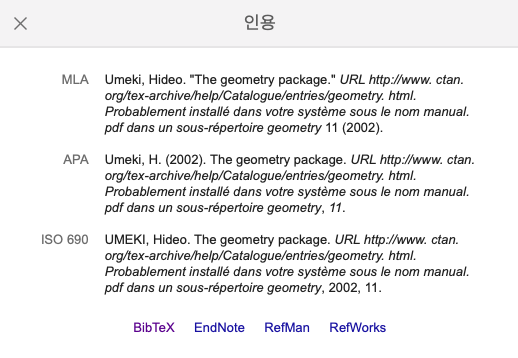
\includegraphics[width=.5 \linewidth]{figures/googlescholar.png}
        \caption{Google Scholar gives BibTex}
    \end{figure}
\end{frame}

\begin{frame}[fragile]
    \frametitle{How can I cite?}
    Only one line command is enough:
    \begin{example}[Citation example]
        \begin{verbatim}
\cite{ref:label}
        \end{verbatim}
    \end{example}
    If you want multiple citation at once, use this command instead:
    \begin{example}[Multiple citation example]
        \begin{verbatim}
\cite{ref:label1, ref:label2}
        \end{verbatim}
    \end{example}
\end{frame}

\begin{frame}[fragile]
    \frametitle{How can I cite? \textit{(cont.)}}
    For a list of references, add these commands where you want:
    \begin{example}[Reference example]
        \begin{verbatim}
\bibliographystyle{apalike}
\bibliography{BibTex_Name}
        \end{verbatim}
    \end{example}
    Moreover, these styles can be used:
    \begin{enumerate}
        \item abbrv
        \item acm
        \item alpha
        \item apalike
        \item ieeetr
        \item plain
        \item siam
    \end{enumerate}

\footnotetext{Reference: http://bit.ly/34of80o}
\end{frame}

\end{document}